\documentclass[dvipdfmx]{beamer}
\usepackage{mySld}

\begin{document}
\title[主記憶]{オペレーティングシステム\\第8章 主記憶(メモリ)}
\date{}

\begin{frame}
  \titlepage
\end{frame}

%=========================================================================
%\begin{frame}
%  \frametitle
%  \tableofcontents
%\end{frame}

\section{ハードウェア構成}
%=========================================================================
\begin{frame}
  \frametitle{主記憶}

{\bf 主記憶}はプログラム,データ,スタック等を置くメモリのこと

CPU と同様に重要な装置

\begin{itemize}
\item TeC の 256バイトの RAM
\item H8/3664 の 32KiB の ROM と2KiB の RAM
\item PC のメモリ(4GiB 〜 16GiB 程度?)
\end{itemize}

この章では,主記憶を管理し複数のプロセスに適切に割り振り,
かつ,プロセス同士が干渉しないように分離する方法を学ぶ.
\end{frame}

%=========================================================================
\begin{frame}
  \frametitle{ハードウェア構成}
  メモリを共有するSMP(Symmetric Multiprocessing)システム
  \begin{center}
    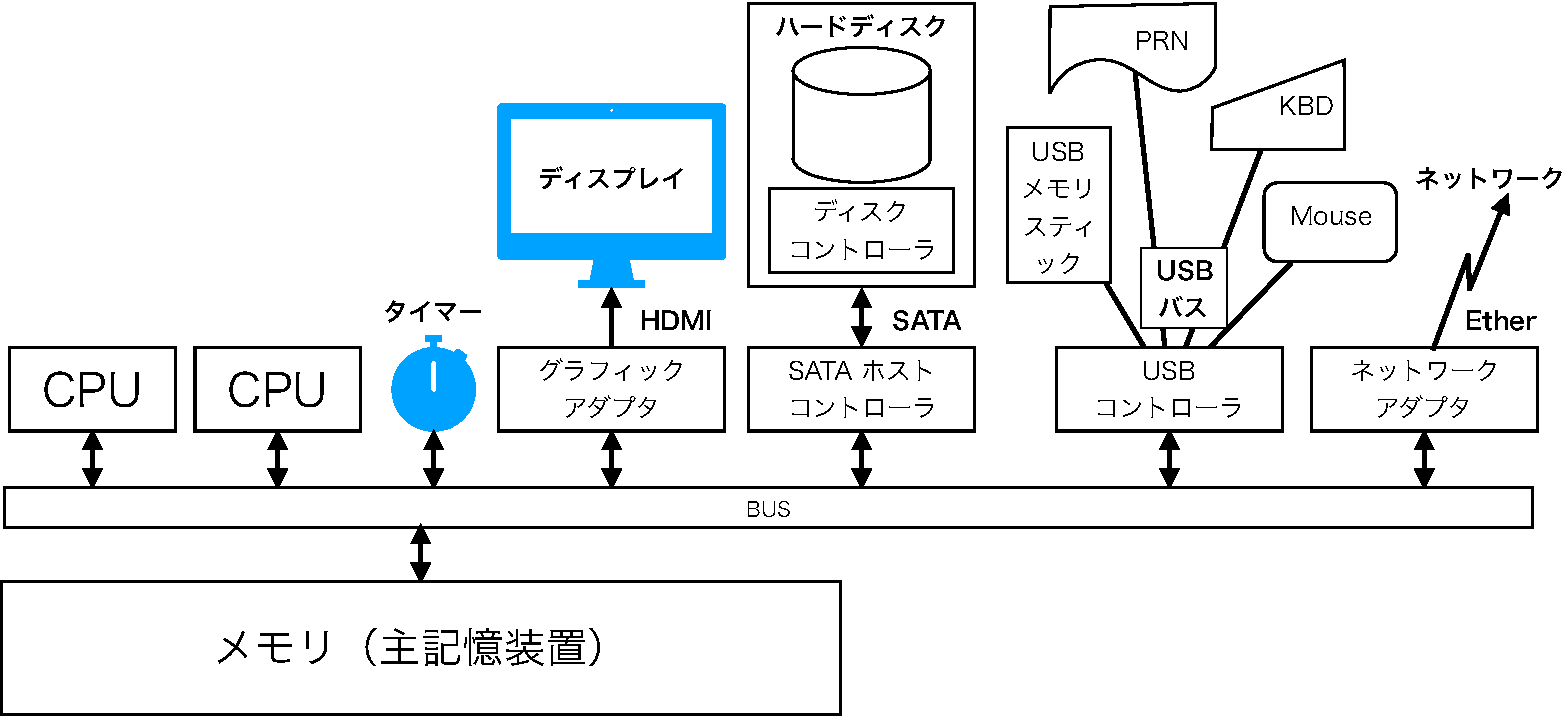
\includegraphics[scale=0.40]{Fig/hardBlock-crop.pdf}\\
    この講義で前提にしているコンピュータの構成
  \end{center}
\end{frame}

%=========================================================================
\begin{frame}
  \frametitle{本章で用いるモデル}
  \begin{center}
    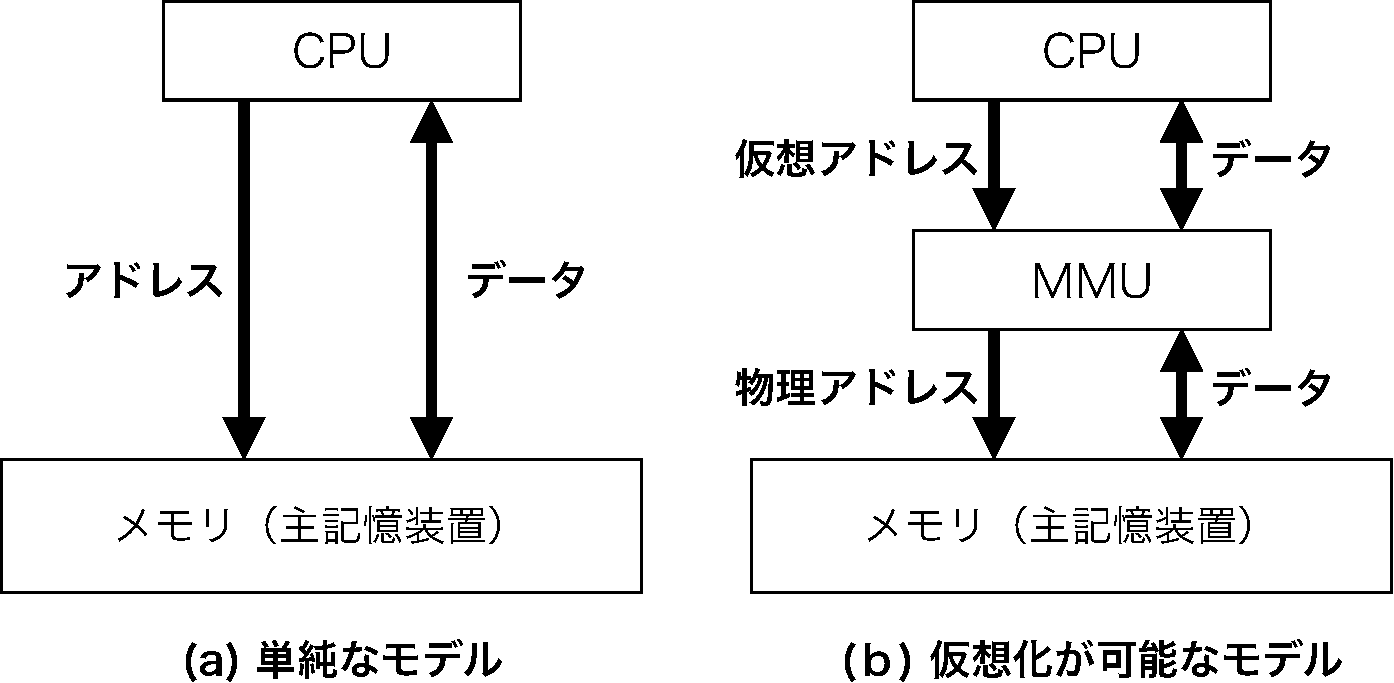
\includegraphics[scale=0.40]{Fig/cpuAndMemory-crop.pdf}\\
  \end{center}
      {\bf MMU(Memory Management Unit:メモリ管理装置)}
      \begin{itemize}
      \item メモリ保護機構,メモリ再配置機構,仮想記憶
      \item 仮想アドレス,物理アドレス
      \end{itemize}
\end{frame}

\section{メモリ保護機構}
%=========================================================================
\begin{frame}
  \frametitle{メモリ保護機構}
  \begin{itemize}
    \item CPUを仮想化した\\
      複数のプロセスを同時にロードし並列実行できるようになった
    \item ユーザプロセスが複数存在する \\
      プロセスが他のプロセスやOSを破壊しないか?\\
      他のプロセスの{\bf メモリを保護}する機構が必要
  \end{itemize}
  プロセスは自身に割当てられたメモリ以外をアクセスできないようにする.
\end{frame}

%=========================================================================
\begin{frame}
  \frametitle{上限・下限レジスタ}
  \begin{itemize}
    \item プロセスがアクセスしても良いアドレスの範囲を設定する.
    \item プロセスのメモリアクセスはアドレスをチェックする(ハード)
    \item レジスタを操作できるのはカーネルだけ.
  \end{itemize}
  \begin{center}
    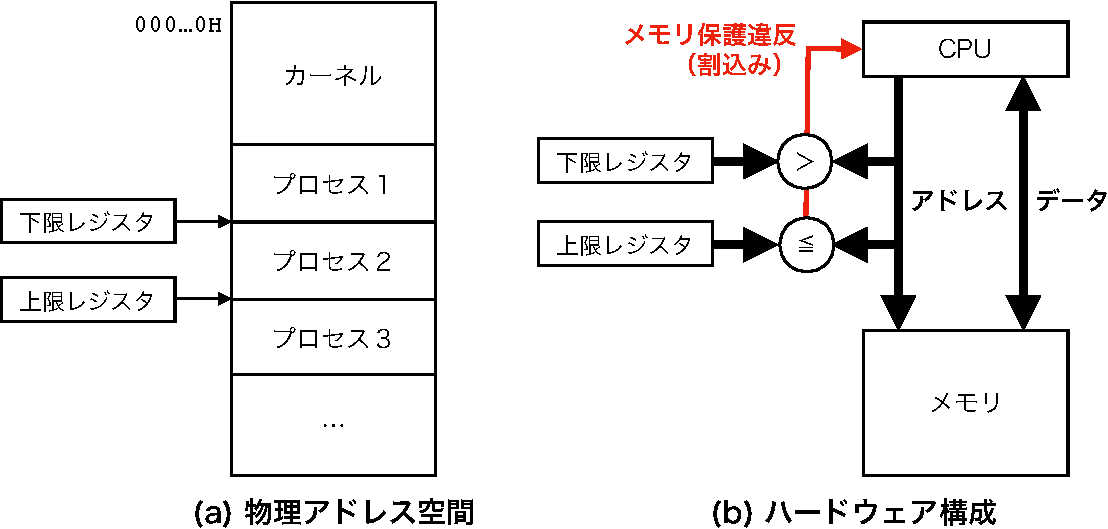
\includegraphics[scale=0.60]{Fig/baseLimitRegister-crop.pdf}\\
  \end{center}
\end{frame}

%=========================================================================
\begin{frame}
  \frametitle{ロック/キー機構}
  \begin{itemize}
    \item メモリをページに分割する(例:64KiBを256ページに)
    \item ページ毎に,アクセスしてよいプロセスとアクセス方法を記録
  \end{itemize}
  \begin{center}
    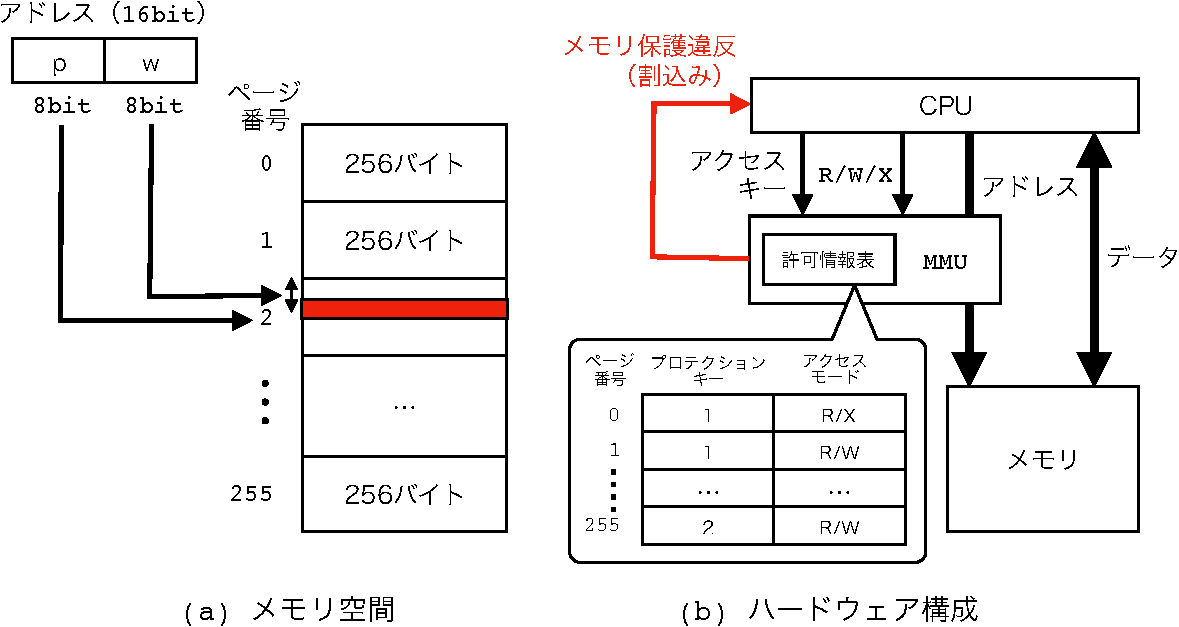
\includegraphics[scale=0.60]{Fig/lockKey-crop.pdf}\\
  \end{center}
\end{frame}

\section{プログラムの再配置}
%=========================================================================
\begin{frame}
  \frametitle{メモリフラグメントとコンパクション}
  \begin{itemize}
    \item 様々なサイズのプロセスが存在する.
    \item プロセスの生成・終了が繰り返される.
    \item メモリフラグメント(断片)が沢山できる.
    \item フラグメントを解消すために{\bf 動的再配置}が必要!
  \end{itemize}
  \begin{center}
    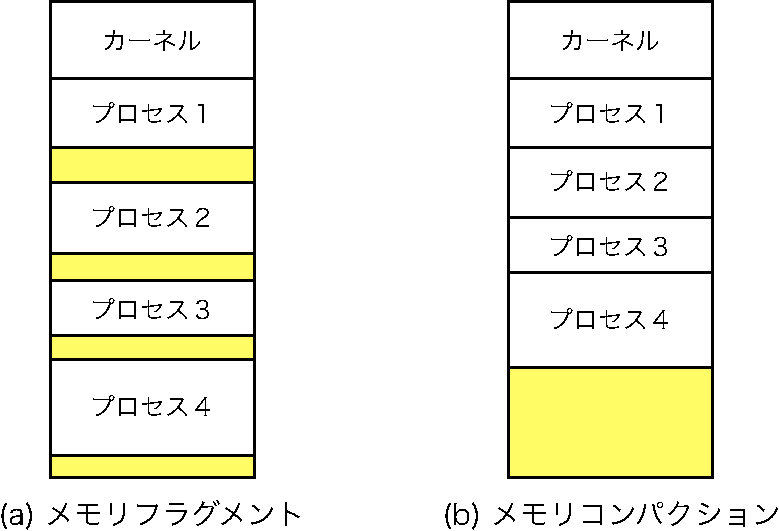
\includegraphics[scale=0.60]{Fig/memoryCompaction-crop.pdf}\\
  \end{center}
\end{frame}

%=========================================================================
\begin{frame}
  \frametitle{再配置可能オブジェクトファイル}
  ロード時に機械語に含まれるアドレスを確定
  \begin{itemize}
    \item コンパイル時にはロードアドレスが分からない.
    \item ロード時にアドレスを確定できる仕組みが必要
    \item 実行可能形式ファイルに機械語と{\bf 再配置表}を格納
    \item ロード時にプログラムやデータに含まれるアドレスを変更
  \end{itemize}
  \vfill
    例:{\tt 1234H}番地にロードされた場合\\
    \begin{quote}
    {\tt JMP 0100H} の機械語は {\tt JMP 1334} に変更
    \end{quote}
\end{frame}

%=========================================================================
\begin{frame}
  \frametitle{動的再配置に応用できるか?}
    この方法では動的再配置までは無理
  \begin{itemize}
    \item CPUレジスタにアドレスがあるかも知れない.
    \item アドレスがスタックにPUSHされているかも.
    \item {\tt malloc()}で確保した領域にも含まれるかも\\
      リスト構造の次のノードへのポインタなど
  \end{itemize}
\end{frame}

%=========================================================================
\begin{frame}
  \frametitle{リロケーションレジスタ}
  \begin{itemize}
    \item 動的再配置を可能にするハードウェア機構
    \item メモリ保護の機能も持つ.
    \item ロードアドレス(B:Base)と大きさ(L:Limit)を記録
  \end{itemize}
  \begin{center}
    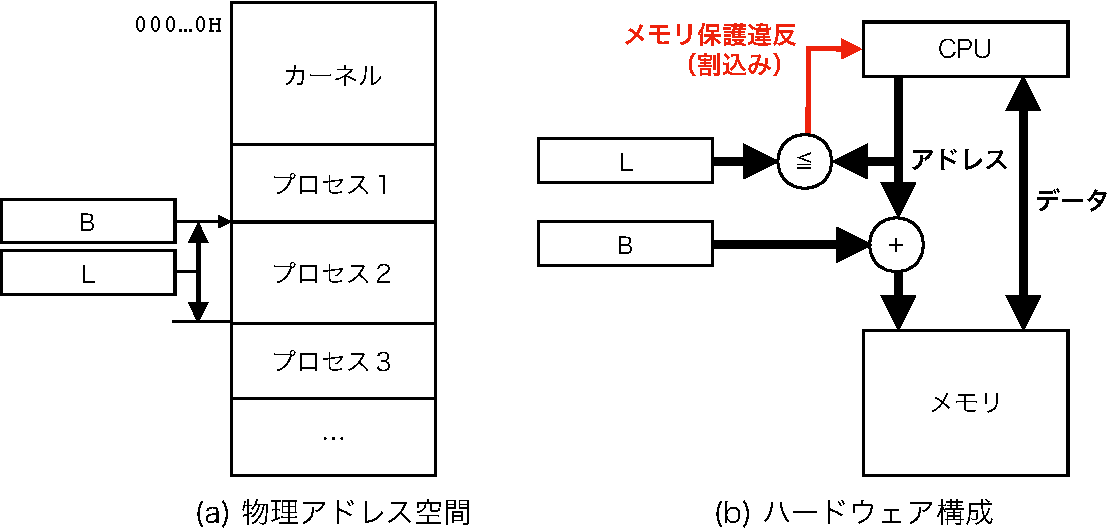
\includegraphics[scale=0.60]{Fig/relocationRegister-crop.pdf}
  \end{center}
\end{frame}

\section{主記憶の仮想化}
%=========================================================================
\begin{frame}
  \frametitle{仮想アドレス空間}
  プロセスは専用の仮想アドレス空間を持っていた(参考)
  \begin{center}
    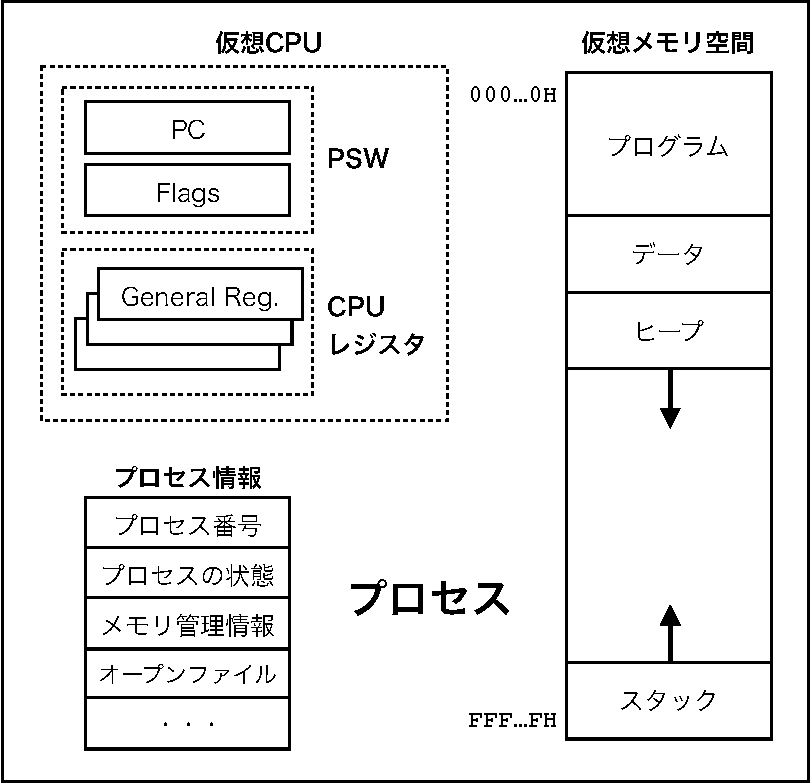
\includegraphics[scale=0.45]{Fig/procOrganization-crop.pdf}
  \end{center}
\end{frame}
%=========================================================================
\begin{frame}
  \frametitle{主記憶の仮想化}
  \begin{itemize}
    \item プロセス毎に独立した仮想アドレス空間を持つ.
    \item 仮想アドレスから物理アドレスにMMUがマッピングする.
    \item 通常は{\bf 多重仮想記憶}方式を用いる.
  \end{itemize}
  \begin{center}
    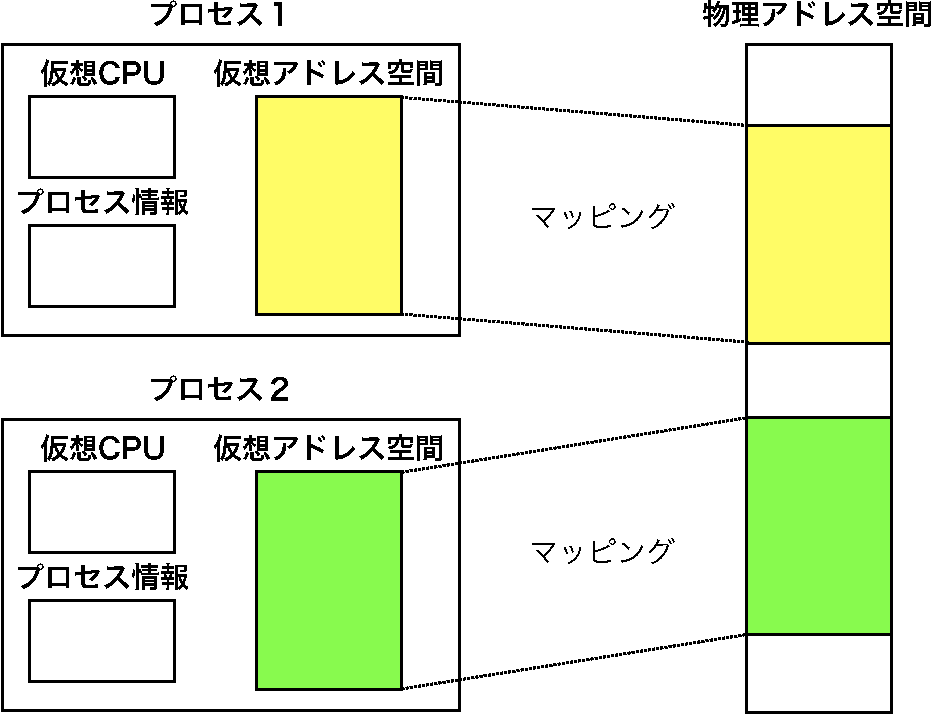
\includegraphics[scale=0.40]{Fig/memorySpaceMapping-crop.pdf}
  \end{center}
\end{frame}

%=========================================================================
\begin{frame}
  \frametitle{仮想化アドレス空間の配置}
  \begin{itemize}
    \item (伝統的な)UNIXの配置をC言語プログラムと対比
    \item ヒープとスタックの間はどれだけ空けておくか?
  \end{itemize}
  \begin{center}
    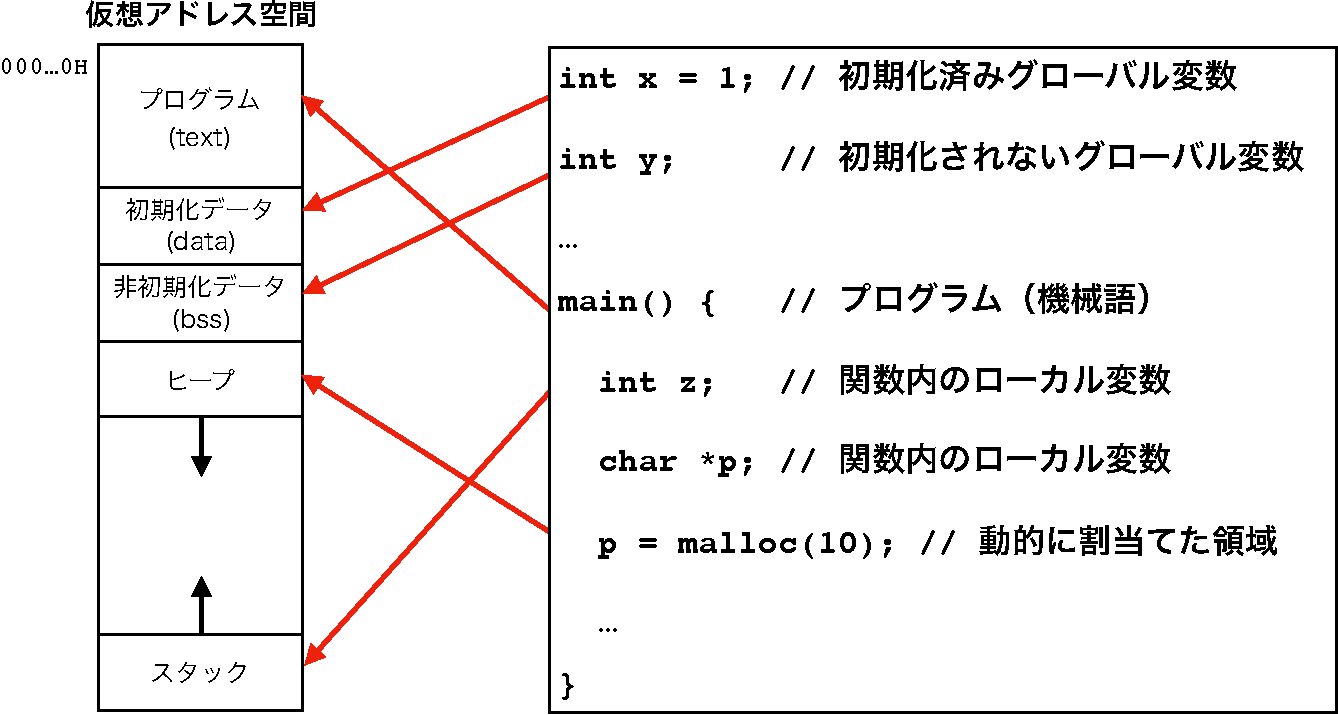
\includegraphics[scale=0.50]{Fig/memoryMapVsClang-crop.pdf}
  \end{center}
\end{frame}

%=========================================================================
\begin{frame}
  \frametitle{前のプログラムをアセンブリ言語に変換したもの}
  \lstinputlisting[numbers=none]{Lst/cmmSample.s}
\end{frame}

\end{document}
